% Options for packages loaded elsewhere
\PassOptionsToPackage{unicode}{hyperref}
\PassOptionsToPackage{hyphens}{url}
%
\documentclass[
]{article}
\usepackage{amsmath,amssymb}
\usepackage{iftex}
\ifPDFTeX
  \usepackage[T1]{fontenc}
  \usepackage[utf8]{inputenc}
  \usepackage{textcomp} % provide euro and other symbols
\else % if luatex or xetex
  \usepackage{unicode-math} % this also loads fontspec
  \defaultfontfeatures{Scale=MatchLowercase}
  \defaultfontfeatures[\rmfamily]{Ligatures=TeX,Scale=1}
\fi
\usepackage{lmodern}
\ifPDFTeX\else
  % xetex/luatex font selection
\fi
% Use upquote if available, for straight quotes in verbatim environments
\IfFileExists{upquote.sty}{\usepackage{upquote}}{}
\IfFileExists{microtype.sty}{% use microtype if available
  \usepackage[]{microtype}
  \UseMicrotypeSet[protrusion]{basicmath} % disable protrusion for tt fonts
}{}
\makeatletter
\@ifundefined{KOMAClassName}{% if non-KOMA class
  \IfFileExists{parskip.sty}{%
    \usepackage{parskip}
  }{% else
    \setlength{\parindent}{0pt}
    \setlength{\parskip}{6pt plus 2pt minus 1pt}}
}{% if KOMA class
  \KOMAoptions{parskip=half}}
\makeatother
\usepackage{xcolor}
\usepackage[margin=1in]{geometry}
\usepackage{color}
\usepackage{fancyvrb}
\newcommand{\VerbBar}{|}
\newcommand{\VERB}{\Verb[commandchars=\\\{\}]}
\DefineVerbatimEnvironment{Highlighting}{Verbatim}{commandchars=\\\{\}}
% Add ',fontsize=\small' for more characters per line
\usepackage{framed}
\definecolor{shadecolor}{RGB}{248,248,248}
\newenvironment{Shaded}{\begin{snugshade}}{\end{snugshade}}
\newcommand{\AlertTok}[1]{\textcolor[rgb]{0.94,0.16,0.16}{#1}}
\newcommand{\AnnotationTok}[1]{\textcolor[rgb]{0.56,0.35,0.01}{\textbf{\textit{#1}}}}
\newcommand{\AttributeTok}[1]{\textcolor[rgb]{0.13,0.29,0.53}{#1}}
\newcommand{\BaseNTok}[1]{\textcolor[rgb]{0.00,0.00,0.81}{#1}}
\newcommand{\BuiltInTok}[1]{#1}
\newcommand{\CharTok}[1]{\textcolor[rgb]{0.31,0.60,0.02}{#1}}
\newcommand{\CommentTok}[1]{\textcolor[rgb]{0.56,0.35,0.01}{\textit{#1}}}
\newcommand{\CommentVarTok}[1]{\textcolor[rgb]{0.56,0.35,0.01}{\textbf{\textit{#1}}}}
\newcommand{\ConstantTok}[1]{\textcolor[rgb]{0.56,0.35,0.01}{#1}}
\newcommand{\ControlFlowTok}[1]{\textcolor[rgb]{0.13,0.29,0.53}{\textbf{#1}}}
\newcommand{\DataTypeTok}[1]{\textcolor[rgb]{0.13,0.29,0.53}{#1}}
\newcommand{\DecValTok}[1]{\textcolor[rgb]{0.00,0.00,0.81}{#1}}
\newcommand{\DocumentationTok}[1]{\textcolor[rgb]{0.56,0.35,0.01}{\textbf{\textit{#1}}}}
\newcommand{\ErrorTok}[1]{\textcolor[rgb]{0.64,0.00,0.00}{\textbf{#1}}}
\newcommand{\ExtensionTok}[1]{#1}
\newcommand{\FloatTok}[1]{\textcolor[rgb]{0.00,0.00,0.81}{#1}}
\newcommand{\FunctionTok}[1]{\textcolor[rgb]{0.13,0.29,0.53}{\textbf{#1}}}
\newcommand{\ImportTok}[1]{#1}
\newcommand{\InformationTok}[1]{\textcolor[rgb]{0.56,0.35,0.01}{\textbf{\textit{#1}}}}
\newcommand{\KeywordTok}[1]{\textcolor[rgb]{0.13,0.29,0.53}{\textbf{#1}}}
\newcommand{\NormalTok}[1]{#1}
\newcommand{\OperatorTok}[1]{\textcolor[rgb]{0.81,0.36,0.00}{\textbf{#1}}}
\newcommand{\OtherTok}[1]{\textcolor[rgb]{0.56,0.35,0.01}{#1}}
\newcommand{\PreprocessorTok}[1]{\textcolor[rgb]{0.56,0.35,0.01}{\textit{#1}}}
\newcommand{\RegionMarkerTok}[1]{#1}
\newcommand{\SpecialCharTok}[1]{\textcolor[rgb]{0.81,0.36,0.00}{\textbf{#1}}}
\newcommand{\SpecialStringTok}[1]{\textcolor[rgb]{0.31,0.60,0.02}{#1}}
\newcommand{\StringTok}[1]{\textcolor[rgb]{0.31,0.60,0.02}{#1}}
\newcommand{\VariableTok}[1]{\textcolor[rgb]{0.00,0.00,0.00}{#1}}
\newcommand{\VerbatimStringTok}[1]{\textcolor[rgb]{0.31,0.60,0.02}{#1}}
\newcommand{\WarningTok}[1]{\textcolor[rgb]{0.56,0.35,0.01}{\textbf{\textit{#1}}}}
\usepackage{graphicx}
\makeatletter
\def\maxwidth{\ifdim\Gin@nat@width>\linewidth\linewidth\else\Gin@nat@width\fi}
\def\maxheight{\ifdim\Gin@nat@height>\textheight\textheight\else\Gin@nat@height\fi}
\makeatother
% Scale images if necessary, so that they will not overflow the page
% margins by default, and it is still possible to overwrite the defaults
% using explicit options in \includegraphics[width, height, ...]{}
\setkeys{Gin}{width=\maxwidth,height=\maxheight,keepaspectratio}
% Set default figure placement to htbp
\makeatletter
\def\fps@figure{htbp}
\makeatother
\setlength{\emergencystretch}{3em} % prevent overfull lines
\providecommand{\tightlist}{%
  \setlength{\itemsep}{0pt}\setlength{\parskip}{0pt}}
\setcounter{secnumdepth}{-\maxdimen} % remove section numbering
\ifLuaTeX
  \usepackage{selnolig}  % disable illegal ligatures
\fi
\usepackage{bookmark}
\IfFileExists{xurl.sty}{\usepackage{xurl}}{} % add URL line breaks if available
\urlstyle{same}
\hypersetup{
  pdftitle={PEC 1},
  pdfauthor={Joan Canseco i Ribas},
  hidelinks,
  pdfcreator={LaTeX via pandoc}}

\title{PEC 1}
\author{Joan Canseco i Ribas}
\date{2024-10-30}

\begin{document}
\maketitle

{
\setcounter{tocdepth}{2}
\tableofcontents
}
\section{Abstract PENDIENTE}\label{abstract-pendiente}

En este proyecto, se ha llevado a cabo un análisis estructurado de datos
metabolómicos para simular un proceso de análisis ómico. El objetivo ha
sido familiarizarse con la organización y manejo de datos ómicos,
aplicando diversas herramientas y métodos que se han ido mostrando
durante la asignatura de ``Análisis de datos ómicos''. Para ello, se ha
seleccionado un conjunto de datos de un estudio en el que se investiga
los metabolitos en respuesta a la cirugía bariátrica en 4 distintos
timepoints en 39 pacientes con más de 10 años de obesidad. Estos 39
pacientes están clasificados en dos grupos, un grupo de pacientes que se
les aplica cirugía by pass (n=26) y otro que se les aplica cirugía
tubular (n=13). Estos datos han sido organizados en un contenedor del
tipo SummarizedExperiment para facilitar el trabajo con este dataset.
Además, se han realizado análisis exploratorios en el que se han
reflejado las características más relevantes del proyecto. También se
han estudiado las características de los principales grupos de estudio,
y \#\#\#\#\#\#\#\#\#\#\#\#\#\#\#\# para verificar cuáles son los
metabolitos que más cambian al aplicar una u otra cirugía. Finalmente,
se ha creado un repositorio del proyecto en Github donde se han subido
todos los documentos del proyecto.

\section{Objetivos del estudio}\label{objetivos-del-estudio}

Los objetivos generales de esta actividad son planificar y ejecutar una
versión simplificada del proceso de análisis de datos ómicos, utilizando
algunas de las herramientas y métodos que se han trabajado en la unidad.
En concreto, se deberá:

\begin{itemize}
\item
  Seleccionar un dataset de un repositorio de github de metabolómica
  \url{https://github.com/nutrimetabolomics/metaboData/}.
\item
  Crear un contenedor del tipo \emph{SummarizedExperiment} que contenga
  los datos y metadatos del dataset.
\item
  Llevar a cabo una exploración del dataset que dé una visión general
  del mismo.
\item
  Elaborar un informe que describa el proceso realizado (este
  documento).
\item
  Crear un repositorio en Github y subir el informe, el objeto
  contenedor con los datos y metadatos, el código R para la exploración
  de los datos, los datos y los metadatos.
\end{itemize}

\section{Materiales y Métodos}\label{materiales-y-muxe9todos}

Esta actividad se ha desarrollado desde un ordenador Windows.

\subsection{Origen y naturaleza de los
datos}\label{origen-y-naturaleza-de-los-datos}

Los datos analizados han sido extraídos del siguiente repositorio
online: \url{https://github.com/nutrimetabolomics/metaboData/} Una vez
accedemos a dicho repositorio, clicamos el botón verde
``\textless\textgreater{} Code'', y clicamos la opción ``Download ZIP''.
Una vez se ha descargado el repositorio en nuestro ordenador, clicamos
botón derecho y seleccionamos ``Extraer todo''. Exploramos los distintos
datasets y seleccionamos el dataset ``2018-MetabotypingPaper'' porque
tiene los documentos bien estructurados y parece que se puede trabajar
bien con él. Cogemos los documentos de dicho dataset y los llevamos a
nuestro directorio de trabajo de la PEC1. Se trata de un dataset de un
estudio de 39 pacientes con más de 10 años de obesidad a los que se les
ha realizado una cirugía bariátrica. Se clasifica el dataset en 2 grupos
según la cirugía bariátrica recibida: grupo ``by pass'' compuesto por 26
pacientes y grupo ``tubular'' compuesto por 13 pacientes. También se
recoge su estado metabólico, en cuanto a si los pacientes estaban sanos
o enfermos metabólicamente en la variable Group. En estos pacientes se
pretende estudiar como evolucionan ciertos metabolitos en 4 distintos
timepoints tras la cirugía según qué cirugía hayan tomado.

\subsection{Herramientas
informáticas}\label{herramientas-informuxe1ticas}

Se han usado principalmente 3 herramientas informáticas y
bioinformáticas para la resolución de la PEC1:

\begin{itemize}
\item
  R y Rstudio: Se ha usado para realizar la exploración del dataset para
  obtener una visión general del mismo. Además, se ha usado para la
  redacción del informe, usando Rmarkdown.
\item
  Bioconductor: Aunque es un paquete de R, lo consideraremos como una
  herramienta independiente para hacer esta explicación. Bioconductor se
  ha usado para crear un contenedor del tipo
  \emph{SummarizedExperiment}.
\item
  Github: Se ha usado para la descarga de los datos (ya se ha indicado
  en la sección previa el procedimiento realizado), y se ha usado para
  presentar los resultados complementarios de la PEC1.
\end{itemize}

\subsection{Creación de un contenedor del tipo
SummarizedExperiment}\label{creaciuxf3n-de-un-contenedor-del-tipo-summarizedexperiment}

Para la creación del contenedor se ha usado Bioconductor dentro de R
(como se ha especificado anteriormente). Los pasos se han especificado
en el apartado de Resultados.

\subsection{Exploración del dataset
PENDIENTE}\label{exploraciuxf3n-del-dataset-pendiente}

Para la exploración de los datos se usará principalmente R y Rstudio. Se
usará en este proyecto dos documentos:

\begin{itemize}
\item
  ``DataValues\_S013.csv'': Se trata del documento donde hay almacenados
  los datos experimentales de los pacientes. Es un data frame con 39
  filas (de 39 pacientes) y 696 variables. De las 696 variables, las 6
  primeras son para identificar a los pacientes (X.1, SUBJECTS, SURGERY,
  AGE, GENDER y Group, en la que X.1 es un duplicado de SUBJECTS, por lo
  que realmente se podría considerar solo las 5 primeras columnas), y el
  resto de variables son los metabolitos tomados en 4 timepoints
  distintos (T0, T2, T4 y T5). Se denota a qué timepoint hace referencia
  cada variable porque al final del nombre de cada variable hay
  especificado el timepoint al que pertenecen con ``\_TX'' (donde X es
  0, 2, 4 o 5).
\item
  ``DataInfo\_S013.csv'': Se trata de un documento donde hay la metadata
  del documento anterior y está organizado de manera distinta. Tiene
  solo 4 columnas (X, es un duplicado de VarName, VarName, contiene el
  nombre de cada una de las variables del documento anterior, varTpe,
  especifica el tipo de variable que es, y Description, especifica qué
  información se recoge en cada variable) y 695 filas, correspondientes
  a las 695 variables del documento anterior (recordemos que eran 696
  pero la primera columna era un duplicado de la segunda columna, por lo
  que son 695 efectivas). Una exploración más exhaustiva será llevada a
  cabo en el apartado de Resultados. En esta exploración se realizará un
  análisis inicial de los datos con dim, head y summary para entender el
  tipo de datos que hay. Además, se realizarán análisis de componentes
  principales (PCA)
\end{itemize}

\subsection{Creación del repositorio
Github}\label{creaciuxf3n-del-repositorio-github}

Primeramente, se ha creado un nuevo repositorio online llamado
``Canseco-i-Ribas-Joan-PEC1'' desde el usuario ``CansecoRibas''. Dentro
del directorio local del proyecto (donde hay todos los documentos que se
han ido mencionando en la parte de ``Materiales y Métodos''), se ha
creado primeramente un proyecto de R, para facilitar el trabajo con
estos documentos. Posteriormente, y desde la Terminal de Rstudio, se ha
creado un repositorio local Git usando el comando ``git init''. Después
se ha establecido conexión con el repositorio online con ``git remote
add origin
\url{https://github.com/CansecoRibas/Canseco-i-Ribas-Joan-PEC1.git}''.
Se han añadido todos los documentos al área de ensayo con ``git add .''
y se ha hecho el primer commit con ``git commit -m `Primer commit del
proyecto'\,''. Seguidamente, se han enviado todos los documentos del
repositorio local al repositorio online con ``git push origin master''.
Una vez se han vinculados los repositorios, se han ido haciendo commits
a medida que se ha ido avanzando en el proyecto. Se puede acceder al
repositorio online desde:
\url{https://github.com/CansecoRibas/Canseco-i-Ribas-Joan-PEC1}

\section{Resultados}\label{resultados}

En este apartado se volcarán los resultados del proyecto.

\subsection{Creación del contenedor del tipo
SummarizedExperiment}\label{creaciuxf3n-del-contenedor-del-tipo-summarizedexperiment}

El primer paso será asegurarnos de que ``BiocManager'' está instalado:

\begin{Shaded}
\begin{Highlighting}[]
\ControlFlowTok{if}\NormalTok{ (}\SpecialCharTok{!}\FunctionTok{requireNamespace}\NormalTok{(}\StringTok{"BiocManager"}\NormalTok{, }\AttributeTok{quietly =} \ConstantTok{TRUE}\NormalTok{)) }\FunctionTok{install.packages}\NormalTok{(}\StringTok{"BiocManager"}\NormalTok{)}
\end{Highlighting}
\end{Shaded}

Posteriormente instalamos desde Bioconductor el paquete
``SummarizedExperiment'' que es el paquete específico para crear el
contendor.

\begin{Shaded}
\begin{Highlighting}[]
\ControlFlowTok{if}\NormalTok{ (}\SpecialCharTok{!}\FunctionTok{requireNamespace}\NormalTok{(}\StringTok{"SummarizedExperiment"}\NormalTok{, }\AttributeTok{quietly =} \ConstantTok{TRUE}\NormalTok{)) BiocManager}\SpecialCharTok{::}\FunctionTok{install}\NormalTok{(}\StringTok{"SummarizedExperiment"}\NormalTok{)}
\end{Highlighting}
\end{Shaded}

Y lo llamamos con library.

\begin{Shaded}
\begin{Highlighting}[]
\FunctionTok{library}\NormalTok{(}\StringTok{"SummarizedExperiment"}\NormalTok{)}
\end{Highlighting}
\end{Shaded}

Ahora cargamos los datos (``DataValues\_S013.csv'') y los metadatos
(``DataInfo\_S013.csv'') del dataset que están dentro de la carpeta
``2018-MetabotypingPaper''.

\begin{Shaded}
\begin{Highlighting}[]
\NormalTok{data\_values }\OtherTok{\textless{}{-}} \FunctionTok{read.csv}\NormalTok{(}\StringTok{"2018{-}MetabotypingPaper/DataValues\_S013.csv"}\NormalTok{)}
\NormalTok{metadata }\OtherTok{\textless{}{-}} \FunctionTok{read.csv}\NormalTok{(}\StringTok{"2018{-}MetabotypingPaper/DataInfo\_S013.csv"}\NormalTok{)}
\end{Highlighting}
\end{Shaded}

Observamos estos dos archivos. Posteriormente ya se hará una mejor
exploración de los datos en próximos apartados. Dejamos este código en
forma de comentarios porque sinó el informe se llena de datos densos.

\begin{Shaded}
\begin{Highlighting}[]
\CommentTok{\#head(data\_values)}
\CommentTok{\#head(metadata)}
\end{Highlighting}
\end{Shaded}

En estos dos documentos hay dos variables iniciales que sobran, ya que
son duplicaciones de las columnas adyacentes. Estas columnas son X.1 en
``DataValues\_S013.csv'' y X en ``DataInfo\_S013.csv'', por lo que las
vamos a eliminar para que no nos molesten.

\begin{Shaded}
\begin{Highlighting}[]
\NormalTok{data\_values\_mod }\OtherTok{\textless{}{-}}\NormalTok{ data\_values[, }\DecValTok{2}\SpecialCharTok{:}\DecValTok{696}\NormalTok{]}
\NormalTok{metadata\_mod }\OtherTok{\textless{}{-}}\NormalTok{ metadata[, }\DecValTok{2}\SpecialCharTok{:}\DecValTok{4}\NormalTok{]}
\end{Highlighting}
\end{Shaded}

Vemos que hay algunas variables identificativas (las 5 primeras) en el
documento ``DataValues\_S013.csv'' y el resto son variables
experimentales. En el documento ``DataInfo\_S013.csv'' se recoge
información de las variables del documento ``DataValues\_S013.csv''.
Algunas de las variables son las mismas pero en distintos timepoints por
lo que vamos a crear una nueva variable que especifique el timepoint. De
esta manera, conseguiremos obtener muestras de manera individual para
las variables. Primero nos aseguramos que los paquetes dplyr y tidyr
estén instalados.

\begin{Shaded}
\begin{Highlighting}[]
\ControlFlowTok{if}\NormalTok{ (}\SpecialCharTok{!}\FunctionTok{requireNamespace}\NormalTok{(}\StringTok{"tidyr"}\NormalTok{, }\AttributeTok{quietly =} \ConstantTok{TRUE}\NormalTok{)) }\FunctionTok{install.packages}\NormalTok{(}\StringTok{"tidyr"}\NormalTok{)}
\ControlFlowTok{if}\NormalTok{ (}\SpecialCharTok{!}\FunctionTok{requireNamespace}\NormalTok{(}\StringTok{"dplyr"}\NormalTok{, }\AttributeTok{quietly =} \ConstantTok{TRUE}\NormalTok{)) }\FunctionTok{install.packages}\NormalTok{(}\StringTok{"dplyr"}\NormalTok{)}
\end{Highlighting}
\end{Shaded}

Los llamamos con library.

\begin{Shaded}
\begin{Highlighting}[]
\FunctionTok{library}\NormalTok{(}\StringTok{"tidyr"}\NormalTok{)}
\FunctionTok{library}\NormalTok{(}\StringTok{"dplyr"}\NormalTok{)}
\end{Highlighting}
\end{Shaded}

Creamos una nueva variable que se llame Timepoint haciendo pivot\_longer
para así obtener las muestras de manera individual que es lo que nos
interesa.

\begin{Shaded}
\begin{Highlighting}[]
\NormalTok{data\_values\_samples }\OtherTok{\textless{}{-}}\NormalTok{ data\_values\_mod }\SpecialCharTok{\%\textgreater{}\%}
  \CommentTok{\# Hacemos pivot\_longer para transformar el df.}
  \FunctionTok{pivot\_longer}\NormalTok{(}
    \AttributeTok{cols =} \DecValTok{6}\SpecialCharTok{:}\DecValTok{695}\NormalTok{, }\CommentTok{\# Seleccionamos las columnas de metabolitos.}
    \AttributeTok{names\_to =} \FunctionTok{c}\NormalTok{(}\StringTok{".value"}\NormalTok{, }\StringTok{"Timepoint"}\NormalTok{), }\CommentTok{\# Extraemos los metabolitos como }
    \CommentTok{\#columnas y establecemos timepoints como nueva columna.}
    \AttributeTok{names\_sep =} \StringTok{"\_T"} \CommentTok{\# Establecemos el separador entre el nombre del metabolito}
    \CommentTok{\# y el timepoint.}
\NormalTok{  ) }\SpecialCharTok{\%\textgreater{}\%}
  \CommentTok{\# Especificamos como queremos que se muestren los timepoints.}
  \FunctionTok{mutate}\NormalTok{(}\AttributeTok{Timepoint =} \FunctionTok{paste0}\NormalTok{(}\StringTok{"T"}\NormalTok{, Timepoint)) }\SpecialCharTok{\%\textgreater{}\%} 
  \FunctionTok{filter}\NormalTok{(}\SpecialCharTok{!}\NormalTok{Timepoint }\SpecialCharTok{==} \StringTok{"TNA"}\NormalTok{) }\CommentTok{\# Eliminamos las filas que se nos han creado por }
\CommentTok{\# error que están completamente vacías.}
\end{Highlighting}
\end{Shaded}

Ahora modificamos el metadata para adecuarlo a las nuevas variables.
Primero añadimos la nueva fila de timepoints creando un nuevo df.

\begin{Shaded}
\begin{Highlighting}[]
\NormalTok{metadata\_timepoints }\OtherTok{\textless{}{-}} \FunctionTok{data.frame}\NormalTok{(}
  \AttributeTok{VarName =} \StringTok{"Timepoint"}\NormalTok{,}
  \AttributeTok{varTpe =} \StringTok{"character"}\NormalTok{,}
  \AttributeTok{Description=} \StringTok{"Punto temporal de recogida de muestra del paciente (0, 2, 4 o 5)"}
\NormalTok{)}
\end{Highlighting}
\end{Shaded}

Modificamos las variables del metadata eliminando ``\_TX'' del final y
eliminamos variables repetidas.

\begin{Shaded}
\begin{Highlighting}[]
\NormalTok{metadata\_metabolites }\OtherTok{\textless{}{-}}\NormalTok{ metadata\_mod }\SpecialCharTok{\%\textgreater{}\%}
  \FunctionTok{mutate}\NormalTok{(}\AttributeTok{VarName =} \FunctionTok{gsub}\NormalTok{(}\StringTok{"\_T[0{-}5]$"}\NormalTok{, }\StringTok{""}\NormalTok{, VarName)) }\SpecialCharTok{\%\textgreater{}\%} \CommentTok{\# Buscamos y eliminamos el "\_TX" del final.}
  \FunctionTok{distinct}\NormalTok{(VarName, }\AttributeTok{.keep\_all =} \ConstantTok{TRUE}\NormalTok{)  }\CommentTok{\# Quitamos las variables repetidas en Varname.}
\end{Highlighting}
\end{Shaded}

Finalmente unimos los dos dfs con rbind.

\begin{Shaded}
\begin{Highlighting}[]
\CommentTok{\# Finalmente unimos los dos dfs con rbind.}
\NormalTok{metadata\_samples }\OtherTok{\textless{}{-}} \FunctionTok{rbind}\NormalTok{(metadata\_timepoints, metadata\_metabolites)}
\end{Highlighting}
\end{Shaded}

Vemos que metadata\_samples tiene las mismas filas que columnas tiene
data\_values\_samples que es lo que estábamos buscando.

\begin{Shaded}
\begin{Highlighting}[]
\FunctionTok{dim}\NormalTok{(metadata\_samples)}
\end{Highlighting}
\end{Shaded}

\begin{verbatim}
## [1] 180   3
\end{verbatim}

\begin{Shaded}
\begin{Highlighting}[]
\FunctionTok{dim}\NormalTok{(data\_values\_samples)}
\end{Highlighting}
\end{Shaded}

\begin{verbatim}
## [1] 156 180
\end{verbatim}

Una vez modificados ambos documentos, nos quedan los datos separados por
muestras individuales cogidas en diferentes timepoints. Ahora ya podemos
crear el objeto ``SummarizedExperiment''. Para ello, seleccionamos las
variables experimentales (a partir de la variable 7 hasta el final) y
creamos una matriz transpuesta llamada ``metabolite\_data'', ya que las
filas deben ser las variables y las columnas deben ser las distintas
muestras.

\begin{Shaded}
\begin{Highlighting}[]
\NormalTok{metabolite\_data }\OtherTok{\textless{}{-}} \FunctionTok{t}\NormalTok{(}\FunctionTok{as.matrix}\NormalTok{(data\_values\_samples[, }\DecValTok{7}\SpecialCharTok{:}\FunctionTok{ncol}\NormalTok{(data\_values\_samples)]))}
\end{Highlighting}
\end{Shaded}

Creamos rowData a partir de la información de la metadata para
especificar la información de las variables experimentales.

\begin{Shaded}
\begin{Highlighting}[]
\NormalTok{rowData }\OtherTok{\textless{}{-}}\NormalTok{ metadata\_samples[}\DecValTok{7}\SpecialCharTok{:}\FunctionTok{nrow}\NormalTok{(metadata\_samples), ]}
\end{Highlighting}
\end{Shaded}

Creamos ColData seleccionando las variables de identificación de los
pacientes.

\begin{Shaded}
\begin{Highlighting}[]
\NormalTok{colData }\OtherTok{\textless{}{-}}\NormalTok{ data\_values\_samples[, }\DecValTok{1}\SpecialCharTok{:}\DecValTok{6}\NormalTok{]}
\end{Highlighting}
\end{Shaded}

Creamos el objeto \emph{SummarizedExperiment} con los 3 componentes que
hemos mencionado.

\begin{Shaded}
\begin{Highlighting}[]
\NormalTok{sum\_exp\_object }\OtherTok{\textless{}{-}} \FunctionTok{SummarizedExperiment}\NormalTok{(}
  \AttributeTok{assays =} \FunctionTok{list}\NormalTok{(}\AttributeTok{counts =}\NormalTok{ metabolite\_data),}
  \AttributeTok{rowData =}\NormalTok{ rowData,}
  \AttributeTok{colData =}\NormalTok{ colData}
\NormalTok{)}
\end{Highlighting}
\end{Shaded}

Vemos qué pinta tiene.

\begin{Shaded}
\begin{Highlighting}[]
\NormalTok{sum\_exp\_object}
\end{Highlighting}
\end{Shaded}

\begin{verbatim}
## class: SummarizedExperiment 
## dim: 174 156 
## metadata(0):
## assays(1): counts
## rownames(174): MEDDM MEDCOL ... X lysoPC.a.C14.0
## rowData names(3): VarName varTpe Description
## colnames: NULL
## colData names(6): SUBJECTS SURGERY ... Group Timepoint
\end{verbatim}

Vemos que es un objeto con 174 filas (variables experimentales de
metabolitos) y 156 columnas, que son las muestras (4 para cada paciente,
ya que son 4 timepoints). Se puede estudiar un poco más el objeto con
las siguientes funciones, pero las dejaremos como comentarios para que
no se muestren unos tochos terribles en el informe.

\begin{Shaded}
\begin{Highlighting}[]
\CommentTok{\#assay(sum\_exp\_object) \# Devuelve la matriz principal de datos.}
\CommentTok{\#rowData(sum\_exp\_object) \# Devuelve un df con información sobre los metabolitos }
\CommentTok{\#(filas de la matriz).}
\CommentTok{\#colData(sum\_exp\_object) \# Devuelve un df con información sobre las muestras }
\CommentTok{\#(columnas de la matriz).}
\end{Highlighting}
\end{Shaded}

Solo queda guardar el objeto tal y como nos pide el enunciado.

\begin{Shaded}
\begin{Highlighting}[]
\FunctionTok{save}\NormalTok{(sum\_exp\_object, }\AttributeTok{file =} \StringTok{"sum\_exp\_object.Rda"}\NormalTok{)}
\end{Highlighting}
\end{Shaded}

\subsection{Exploración del dataset
PENDIENTE}\label{exploraciuxf3n-del-dataset-pendiente-1}

Empezamos con el análisis de ambos documentos, ``DataValues\_S013.csv''
y ``DataInfo\_S013.csv''. Como se ha indicado anteriormente, el primero
contiene los datos en relación a los metabolitos recogidos en muestras
de 4 distintos timepoints de 39 pacientes, y el segundo contiene la
explicación de las características de las variables y su información.
Por lo que nos fijaremos para hacer los análisis en el primer documento
(``DataValues\_S013.csv'').

\subsubsection{Análisis preliminar}\label{anuxe1lisis-preliminar}

Primero haremos una exploración inicial. Cogeremos el documento
data\_values\_samples, en el que hemos transformado los datos para que
las filas sean las muestras recogidas (y no los pacientes como antes).
Verificaremos las dimensiones del documento para ver si lo que se cumple
es cierto.

\begin{Shaded}
\begin{Highlighting}[]
\FunctionTok{dim}\NormalTok{(data\_values\_samples)}
\end{Highlighting}
\end{Shaded}

\begin{verbatim}
## [1] 156 180
\end{verbatim}

Vemos que es un documento con 156 filas (correspondiente a los 4
timepoints de los 39 pacientes) y 180 columnas (correspondientes a las
variables de estudio). Hacemos ahora un resumen estadístico muy básico
de las 180 variables para ver qué valores toman y qué tipos de variables
tenemos. Es un poco complicado trabajar con este número tan elevado de
variables ya que los outputs son enormes, por lo que en este caso
tampoco vamos a mostrar el resultado.

\begin{Shaded}
\begin{Highlighting}[]
\CommentTok{\#summary(data\_values\_samples)}
\end{Highlighting}
\end{Shaded}

También es importante verificar los missings de los datos. Vamos a mirar
cuantos missings hay por cada variable.

\begin{Shaded}
\begin{Highlighting}[]
\FunctionTok{colSums}\NormalTok{(}\FunctionTok{is.na}\NormalTok{(data\_values\_samples))}
\end{Highlighting}
\end{Shaded}

\begin{verbatim}
##       SUBJECTS        SURGERY            AGE         GENDER          Group 
##              0              0              0              0              0 
##      Timepoint          MEDDM         MEDCOL         MEDINF         MEDHTA 
##              0             13             13             15             13 
##            GLU            INS           HOMA          HBA1C HBA1C.mmol.mol 
##             11             14             14             91             91 
##           PESO            bmi             CC           CINT            CAD 
##             10             10             24             14             14 
##            TAD            TAS             TG            COL            LDL 
##             25             25             11             11             18 
##            HDL           VLDL            PCR            LEP          ADIPO 
##             13             49             68             68             71 
##            GOT            GPT            GGT          URICO          CREAT 
##             12             12             15             16             15 
##           UREA         HIERRO         TRANSF           FERR            Ile 
##             15             13             25             16             18 
##            Leu            Val            Ala            Pro            Gly 
##             18             18             18             18             18 
##            Ser            Trp            Phe            Met            Orn 
##             18             18             18             18             18 
##            Arg            His            Asn            Asp            Glu 
##             18             18             18             18             18 
##            Gln            Cit            Tyr            Thr            Lys 
##             18             18             18             18             18 
##     Creatinine     Kynurenine     Putrescine      Sarcosine      Serotonin 
##             18             18             21             18             18 
##        Taurine           SDMA             C0             C2          C3.OH 
##             18             18             18             18             18 
##   C6..C4.1.DC.  C5.DC..C6.OH.          C7.DC             C8            C10 
##             18             18             18             18             18 
##          C10.1          C10.2          C14.1          C14.2          C16.1 
##             18             18             18             18             18 
##          C16.2       C16.2.OH          C18.1       C18.1.OH          C18.2 
##             18             18             18             18             18 
## lysoPC.a.C16.0 lysoPC.a.C16.1 lysoPC.a.C17.0 lysoPC.a.C18.0 lysoPC.a.C18.1 
##             18             18             18             18             18 
## lysoPC.a.C18.2 lysoPC.a.C20.3 lysoPC.a.C20.4 lysoPC.a.C24.0 lysoPC.a.C26.0 
##             18             18             18             18             18 
## lysoPC.a.C26.1 lysoPC.a.C28.0 lysoPC.a.C28.1    PC.aa.C24.0    PC.aa.C28.1 
##             18             18             18             18             18 
##    PC.aa.C30.0    PC.aa.C32.0    PC.aa.C32.1    PC.aa.C32.3    PC.aa.C34.1 
##             18             18             18             18             18 
##    PC.aa.C34.2    PC.aa.C34.3    PC.aa.C34.4    PC.aa.C36.0    PC.aa.C36.1 
##             18             18             18             18             18 
##    PC.aa.C36.2    PC.aa.C36.3    PC.aa.C36.4    PC.aa.C36.5    PC.aa.C38.0 
##             18             18             18             18             18 
##    PC.aa.C38.1    PC.aa.C38.3    PC.aa.C38.4    PC.aa.C38.5    PC.aa.C38.6 
##             18             18             18             18             18 
##    PC.aa.C40.1    PC.aa.C40.2    PC.aa.C40.3    PC.aa.C40.4    PC.aa.C40.5 
##             18             18             18             18             18 
##    PC.aa.C40.6    PC.aa.C42.0    PC.aa.C42.1    PC.aa.C42.2    PC.aa.C42.4 
##             18             18             18             18             18 
##    PC.aa.C42.5    PC.aa.C42.6    PC.ae.C30.0    PC.ae.C32.1    PC.ae.C32.2 
##             18             18             18             18             18 
##    PC.ae.C34.0    PC.ae.C34.1    PC.ae.C34.2    PC.ae.C34.3    PC.ae.C36.0 
##             18             18             18             18             18 
##    PC.ae.C36.1    PC.ae.C36.2    PC.ae.C36.3    PC.ae.C36.4    PC.ae.C36.5 
##             18             18             18             18             18 
##    PC.ae.C38.0    PC.ae.C38.2    PC.ae.C38.3    PC.ae.C38.4    PC.ae.C38.5 
##             18             18             18             18             18 
##    PC.ae.C38.6    PC.ae.C40.1    PC.ae.C40.2    PC.ae.C40.3    PC.ae.C40.4 
##             18             18             18             18             18 
##    PC.ae.C40.5    PC.ae.C40.6    PC.ae.C42.1    PC.ae.C42.2    PC.ae.C42.3 
##             18             18             18             18             18 
##    PC.ae.C42.4    PC.ae.C42.5    PC.ae.C44.3    PC.ae.C44.4    PC.ae.C44.5 
##             18             18             18             18             18 
##    PC.ae.C44.6  SM..OH..C14.1  SM..OH..C16.1  SM..OH..C22.1  SM..OH..C22.2 
##             18             18             18             18             18 
##  SM..OH..C24.1       SM.C16.0       SM.C16.1       SM.C18.0       SM.C18.1 
##             18             18             18             18             18 
##       SM.C20.2       SM.C24.0       SM.C24.1              X lysoPC.a.C14.0 
##             18             18             18            156            118
\end{verbatim}

Vemos que las variables identificativas están completas, mientras que
todas las variables de metabolitos tienen algún missing, aunque en
general son pocos (la mayoría tienen menos de 19 missings de 156 valores
totales). Además, hay una variable ``X'' que son todo missings.

\subsubsection{Análisis de los
pacientes}\label{anuxe1lisis-de-los-pacientes}

Como hay muchas variables de metabolitos, haremos una exploración
inicial de las variables identificativas de los pacientes, que, como
hemos dicho son las 5 primeras variables (excluyendo la variable
Timepoint que en este caso no tiene mucho sentido mantenerla porque hace
referencia a las muestras).

\begin{Shaded}
\begin{Highlighting}[]
\NormalTok{data\_values\_patients }\OtherTok{\textless{}{-}}\NormalTok{ data\_values\_samples }\SpecialCharTok{\%\textgreater{}\%} 
  \FunctionTok{select}\NormalTok{(}\StringTok{"SUBJECTS"}\NormalTok{, }\StringTok{"SURGERY"}\NormalTok{, }\StringTok{"AGE"}\NormalTok{, }\StringTok{"GENDER"}\NormalTok{, }\StringTok{"Group"}\NormalTok{) }\SpecialCharTok{\%\textgreater{}\%} \CommentTok{\# Seleccionamos columnas}
  \FunctionTok{distinct}\NormalTok{() }\CommentTok{\# Eliminamos duplicados de pacientes}
\end{Highlighting}
\end{Shaded}

Verificamos que tenemos 39 pacientes en este df.

\begin{Shaded}
\begin{Highlighting}[]
\FunctionTok{nrow}\NormalTok{(data\_values\_patients)}
\end{Highlighting}
\end{Shaded}

\begin{verbatim}
## [1] 39
\end{verbatim}

Verificamos las variables que deban ser factors realmente sean factors.

\begin{Shaded}
\begin{Highlighting}[]
\NormalTok{data\_values\_patients}\SpecialCharTok{$}\NormalTok{SURGERY }\OtherTok{\textless{}{-}} \FunctionTok{factor}\NormalTok{(data\_values\_patients}\SpecialCharTok{$}\NormalTok{SURGERY)}
\NormalTok{data\_values\_patients}\SpecialCharTok{$}\NormalTok{GENDER }\OtherTok{\textless{}{-}} \FunctionTok{factor}\NormalTok{(data\_values\_patients}\SpecialCharTok{$}\NormalTok{GENDER)}
\NormalTok{data\_values\_patients}\SpecialCharTok{$}\NormalTok{Group }\OtherTok{\textless{}{-}} \FunctionTok{factor}\NormalTok{(data\_values\_patients}\SpecialCharTok{$}\NormalTok{Group)}
\end{Highlighting}
\end{Shaded}

Ahora podemos hacer estadística básica con estos datos de los pacientes.
Los datos realmente importantes de este df se encuentran en las
variables ``SURGERY'', ``AGE'', ``GENDER'' y ``Group'', ya que
``SUBJECTS'' solo hace referencia al número de paciente. La variable
``AGE'' la veremos con un histograma mientras que los factores los
veremos con diagramas de barras.

\begin{Shaded}
\begin{Highlighting}[]
\FunctionTok{par}\NormalTok{(}\AttributeTok{mfrow =} \FunctionTok{c}\NormalTok{(}\DecValTok{2}\NormalTok{,}\DecValTok{2}\NormalTok{)) }\CommentTok{\# Así podemos ver los 4 gráficos a la vez.}
\CommentTok{\# Histograma de la edad.}
\FunctionTok{hist}\NormalTok{(data\_values\_patients}\SpecialCharTok{$}\NormalTok{AGE, }
     \AttributeTok{main=}\StringTok{"Distribución de edades"}\NormalTok{, }
     \AttributeTok{col=}\StringTok{"blue"}\NormalTok{, }
     \AttributeTok{xlab=}\StringTok{"Edad en años"}\NormalTok{,}
     \AttributeTok{ylab=}\StringTok{"Frecuencia"}\NormalTok{)}

\CommentTok{\# Diagrama de barras para el género.}
\FunctionTok{barplot}\NormalTok{(}\FunctionTok{table}\NormalTok{(data\_values\_patients}\SpecialCharTok{$}\NormalTok{GENDER), }
        \AttributeTok{main=}\StringTok{"Distribución por género"}\NormalTok{, }
        \AttributeTok{col=}\StringTok{"red"}\NormalTok{, }
        \AttributeTok{xlab=}\StringTok{"Género"}\NormalTok{,}
        \AttributeTok{ylim=}\FunctionTok{c}\NormalTok{(}\DecValTok{0}\NormalTok{,}\DecValTok{30}\NormalTok{))}

\CommentTok{\# Diagrama de barras para el grupo.}
\FunctionTok{barplot}\NormalTok{(}\FunctionTok{table}\NormalTok{(data\_values\_patients}\SpecialCharTok{$}\NormalTok{Group), }
        \AttributeTok{main=}\StringTok{"Distribución por grupo"}\NormalTok{, }
        \AttributeTok{col=}\StringTok{"green"}\NormalTok{, }
        \AttributeTok{xlab=}\StringTok{"Grupo"}\NormalTok{,}
        \AttributeTok{ylim=}\FunctionTok{c}\NormalTok{(}\DecValTok{0}\NormalTok{,}\DecValTok{30}\NormalTok{))}

\CommentTok{\# Diagrama de barras para la cirugía.}
\FunctionTok{barplot}\NormalTok{(}\FunctionTok{table}\NormalTok{(data\_values\_patients}\SpecialCharTok{$}\NormalTok{SURGERY), }
        \AttributeTok{main=}\StringTok{"Distribución por cirugía"}\NormalTok{, }
        \AttributeTok{col=}\StringTok{"pink"}\NormalTok{, }
        \AttributeTok{xlab=}\StringTok{"Cirugía"}\NormalTok{,}
        \AttributeTok{ylim=}\FunctionTok{c}\NormalTok{(}\DecValTok{0}\NormalTok{,}\DecValTok{30}\NormalTok{))}
\end{Highlighting}
\end{Shaded}

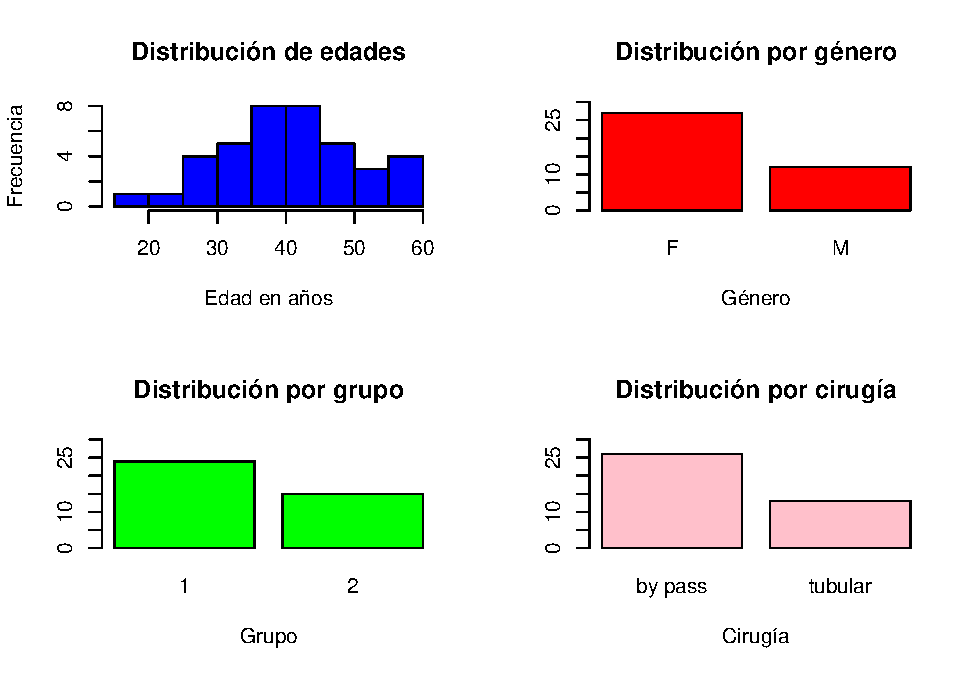
\includegraphics{Informe-PEC1_files/figure-latex/unnamed-chunk-27-1.pdf}

Estos gráficos muestran que la mayoría de edades de los participantes
están entre los 30 y los 50 años, que hay el doble de mujeres que de
hombres, que hay más componentes del grupo 1 que del grupo 2 y que hay
más pacientes con cirugía by pass que tubular. Ahora miraremos la
relación entre la variable SURGERY (la variable que indica el tipo de
cirugía que ha tomado cada paciente) y las demás, ya que la variable
SURGERY es la variable clave del estudio.

\begin{Shaded}
\begin{Highlighting}[]
\CommentTok{\# Separamos los datos según la variable SURGERY.}
\NormalTok{split\_data }\OtherTok{\textless{}{-}} \FunctionTok{split}\NormalTok{(data\_values\_patients, data\_values\_patients}\SpecialCharTok{$}\NormalTok{SURGERY)}

\CommentTok{\# Redistribuimos el espacio gráfico.}
\FunctionTok{par}\NormalTok{(}\AttributeTok{mfrow =} \FunctionTok{c}\NormalTok{(}\DecValTok{2}\NormalTok{, }\DecValTok{3}\NormalTok{)) }

\CommentTok{\# Hacemos loop.}
\ControlFlowTok{for}\NormalTok{ (surgery\_status }\ControlFlowTok{in} \FunctionTok{names}\NormalTok{(split\_data)) \{}
\NormalTok{  data\_subset }\OtherTok{\textless{}{-}}\NormalTok{ split\_data[[surgery\_status]]}
  
  \CommentTok{\# Histograma de la edad.}
  \FunctionTok{hist}\NormalTok{(data\_subset}\SpecialCharTok{$}\NormalTok{AGE,}
       \AttributeTok{main=}\FunctionTok{paste}\NormalTok{(}\StringTok{"Edades ("}\NormalTok{, surgery\_status, }\StringTok{")"}\NormalTok{), }
       \AttributeTok{col=}\StringTok{"blue"}\NormalTok{, }
       \AttributeTok{xlab=}\StringTok{"Edad en años"}\NormalTok{,}
       \AttributeTok{ylab=}\StringTok{"Frecuencia"}\NormalTok{)}
  
  \CommentTok{\# Diagrama de barras para el género.}
  \FunctionTok{barplot}\NormalTok{(}\FunctionTok{table}\NormalTok{(data\_subset}\SpecialCharTok{$}\NormalTok{GENDER), }
          \AttributeTok{main=}\FunctionTok{paste}\NormalTok{(}\StringTok{"Género ("}\NormalTok{, surgery\_status, }\StringTok{")"}\NormalTok{), }
          \AttributeTok{col=}\StringTok{"red"}\NormalTok{, }
          \AttributeTok{xlab=}\StringTok{"Género"}\NormalTok{,}
          \AttributeTok{ylim=}\FunctionTok{c}\NormalTok{(}\DecValTok{0}\NormalTok{,}\DecValTok{30}\NormalTok{))}
  
  \CommentTok{\# Diagrama de barras para el grupo.}
  \FunctionTok{barplot}\NormalTok{(}\FunctionTok{table}\NormalTok{(data\_subset}\SpecialCharTok{$}\NormalTok{Group), }
          \AttributeTok{main=}\FunctionTok{paste}\NormalTok{(}\StringTok{"Grupo ("}\NormalTok{, surgery\_status, }\StringTok{")"}\NormalTok{), }
          \AttributeTok{col=}\StringTok{"green"}\NormalTok{, }
          \AttributeTok{xlab=}\StringTok{"Grupo"}\NormalTok{,}
          \AttributeTok{ylim=}\FunctionTok{c}\NormalTok{(}\DecValTok{0}\NormalTok{,}\DecValTok{30}\NormalTok{))}
\NormalTok{\}}
\end{Highlighting}
\end{Shaded}

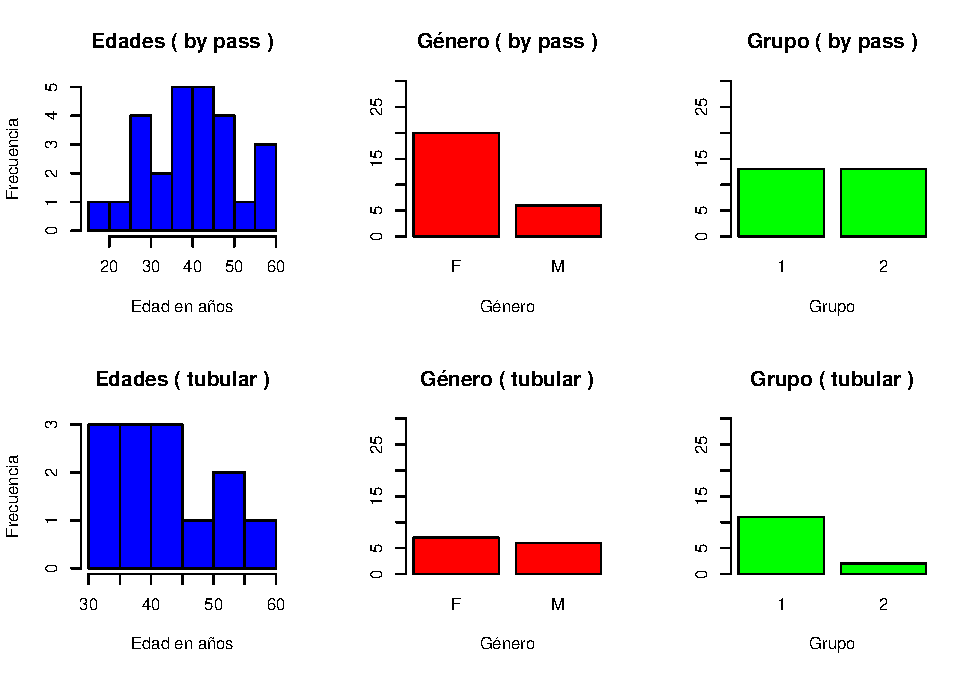
\includegraphics{Informe-PEC1_files/figure-latex/unnamed-chunk-28-1.pdf}

Vemos que los grupos son bastante diferentes entre ellos, también
probablemente porque la n es relativamente pequeña, aun que no sabemos
si puede afectar a nuestros resultados.

\subsubsection{Análisis}\label{anuxe1lisis}

Se propone dilucidar que metabolitos varían más desde el T=0 hasta el
T=5 (el último timepoint que hay) en cada una de las cirugías (bypass y
tubular). Filtramos primero los timepoints 0 y 5.

\begin{Shaded}
\begin{Highlighting}[]
\NormalTok{data\_values\_timepoints }\OtherTok{\textless{}{-}}\NormalTok{ data\_values\_samples[data\_values\_samples}\SpecialCharTok{$}\NormalTok{Timepoint }\SpecialCharTok{\%in\%} \FunctionTok{c}\NormalTok{(}\StringTok{"T0"}\NormalTok{, }\StringTok{"T5"}\NormalTok{), ]}
\end{Highlighting}
\end{Shaded}

Creamos un df para almacenar las diferencias de metaboitos entre
timepoints.

\begin{Shaded}
\begin{Highlighting}[]
\NormalTok{data\_values\_difference }\OtherTok{\textless{}{-}} \FunctionTok{data.frame}\NormalTok{()}
\end{Highlighting}
\end{Shaded}

Carlcculamos la diferencia entre metabolitos para cada paciente.

\begin{Shaded}
\begin{Highlighting}[]
\ControlFlowTok{for}\NormalTok{ (patient }\ControlFlowTok{in} \FunctionTok{unique}\NormalTok{(data\_values\_timepoints}\SpecialCharTok{$}\NormalTok{SUBJECTS)) \{}
\NormalTok{  patient\_data }\OtherTok{\textless{}{-}}\NormalTok{ data\_values\_timepoints[data\_values\_timepoints}\SpecialCharTok{$}\NormalTok{SUBJECTS }\SpecialCharTok{==}\NormalTok{ patient, ]}
  
  \CommentTok{\# Solo si hay valores en ambos timepoints.}
  \ControlFlowTok{if}\NormalTok{ (}\FunctionTok{all}\NormalTok{(}\FunctionTok{c}\NormalTok{(}\DecValTok{0}\NormalTok{, }\DecValTok{4}\NormalTok{) }\SpecialCharTok{\%in\%}\NormalTok{ patient\_data}\SpecialCharTok{$}\NormalTok{Timepoint)) \{}
    \CommentTok{\# Obtener las filas para timepoint 0 y 5.}
\NormalTok{    tp0 }\OtherTok{\textless{}{-}}\NormalTok{ patient\_data[patient\_data}\SpecialCharTok{$}\NormalTok{Timepoint }\SpecialCharTok{==} \StringTok{"T0"}\NormalTok{, ]}
\NormalTok{    tp4 }\OtherTok{\textless{}{-}}\NormalTok{ patient\_data[patient\_data}\SpecialCharTok{$}\NormalTok{Timepoint }\SpecialCharTok{==} \StringTok{"T5"}\NormalTok{, ]}
    
    \CommentTok{\# Calcular las diferencias de cada metabolito entre tp4 y tp0.}
\NormalTok{    diff\_row }\OtherTok{\textless{}{-}}\NormalTok{ tp5}
\NormalTok{    diff\_row[ , }\FunctionTok{names}\NormalTok{(tp5) }\SpecialCharTok{\%in\%} \FunctionTok{colnames}\NormalTok{(data\_values\_samples)[}\SpecialCharTok{{-}}\NormalTok{(}\DecValTok{1}\SpecialCharTok{:}\DecValTok{3}\NormalTok{)]] }\OtherTok{\textless{}{-}}\NormalTok{ tp4[ , }\SpecialCharTok{{-}}\NormalTok{(}\DecValTok{1}\SpecialCharTok{:}\DecValTok{3}\NormalTok{)] }\SpecialCharTok{{-}}\NormalTok{ tp0[ , }\SpecialCharTok{{-}}\NormalTok{(}\DecValTok{1}\SpecialCharTok{:}\DecValTok{3}\NormalTok{)]}
\NormalTok{    diff\_row}\SpecialCharTok{$}\NormalTok{Timepoint }\OtherTok{\textless{}{-}} \StringTok{"Difference"}
    
    \CommentTok{\# Añadir a data\_values\_difference}
\NormalTok{    data\_values\_difference }\OtherTok{\textless{}{-}} \FunctionTok{rbind}\NormalTok{(data\_values\_difference, diff\_row)}
\NormalTok{  \}}
\NormalTok{\}}

\CommentTok{\# Comparar diferencias entre tipos de cirugía}
\CommentTok{\# Supongamos que los metabolitos son: Metabolite1, Metabolite2, ..., MetaboliteN}
\NormalTok{metabolite\_columns }\OtherTok{\textless{}{-}} \FunctionTok{colnames}\NormalTok{(data\_values\_samples)[}\SpecialCharTok{{-}}\NormalTok{(}\DecValTok{1}\SpecialCharTok{:}\DecValTok{3}\NormalTok{)] }\CommentTok{\# Asume que las primeras tres columnas son IDs y Timepoint}

\CommentTok{\#for (metabolite in metabolite\_columns) \{}
  \CommentTok{\# Comparación estadística para el metabolito entre tipos de cirugía}
  \CommentTok{\#bypass\_values \textless{}{-} data\_values\_difference[data\_values\_difference$Surgery\_Type == "bypass", metabolite]}
  \CommentTok{\#tubular\_values \textless{}{-} data\_values\_difference[data\_values\_difference$Surgery\_Type == "tubular", metabolite]}
  
  \CommentTok{\# Prueba estadística (ajusta a t{-}test o Wilcoxon según la distribución de los datos)}
  \CommentTok{\#test\_result \textless{}{-} t.test(bypass\_values, tubular\_values)}
\CommentTok{\#\}}
\end{Highlighting}
\end{Shaded}

\section{Discusión y limitaciones y conclusiones del estudio
PENDIENTE}\label{discusiuxf3n-y-limitaciones-y-conclusiones-del-estudio-pendiente}

\end{document}
